\documentclass[crop,tikz]{standalone}

\usetikzlibrary{shadows.blur}
\usetikzlibrary{shapes.symbols}
\usetikzlibrary{arrows.meta}

\begin{document}
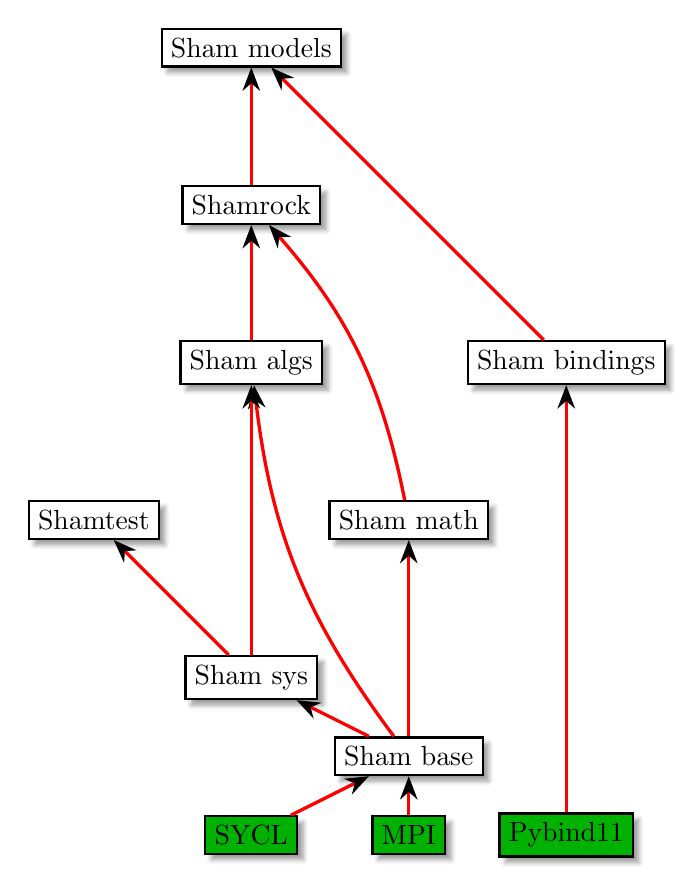
\begin{tikzpicture}

\begin{scope}[
    every node/.style={
        thick,
        draw,
        blur shadow={shadow blur steps=5},
        fill=white}]

    \node (shamsys) at (0,0) {Sham sys};
    \node (shambase) at (2,-1) {Sham base};
    \node (shammath) at (2,2) {Sham math};
    \node (shamalgs) at (0,4) {Sham algs};
    \node (shamrock) at (0,6) {Shamrock};

    \node (shamtest) at (-2,2) {Shamtest};
    %\node (tests) at (0,6) {Tests};
    \node (shammodels) at (0,8) {Sham models};
    \node (shambindings) at (4,4) {Sham bindings};
\end{scope}


\begin{scope}[
    every node/.style={
        thick,
        draw,
        fill=black!30!green,
        blur shadow={shadow blur steps=5}}]

    \node (SYCL) at (0,-2) {SYCL};
    \node (MPI) at (2,-2) {MPI};
    \node (Pybind11) at (4,-2) {Pybind11};
\end{scope}


\begin{scope}[>={Stealth[black]},
              every node/.style={fill=white,circle},
              every edge/.style={draw=red,very thick}]

    \path [->] (SYCL) edge  (shambase); 
    \path [->] (MPI) edge  (shambase);  
    \path [->] (shambase) edge  (shamsys);  
    \path [->] (shambase) edge  (shammath);  
    \path [->] (shambase) edge[bend left=15]  (shamalgs);   
    \path [->] (shamsys) edge  (shamalgs);  
    \path [->] (shamsys) edge  (shamtest);  
    \path [->] (shamalgs) edge  (shamrock); 
    \path [->] (shammath) edge[bend right=15]  (shamrock);  
    \path [->] (shamrock) edge  (shammodels); 
    \path [->] (shambindings) edge  (shammodels);   
    \path [->] (Pybind11) edge  (shambindings);    

\end{scope}
\end{tikzpicture}
\end{document}